%!TEX root = ../report.tex
\documentclass[report.tex]{subfiles}
\begin{document}
    \chapter{Solution}
    We discussed various kind of controllers in chapter \ref{State of the Art} session \ref{Controller} and the background knowledge of Popov-Vereshchagin hybrid solver in chapter \ref{Background}.In this chapter The proposed robot archtechture session will present how the forementioned sovler and controller implement on the robot. Session extension of Robif2b will discuss how to modify Robif2b such that the communication between robot and the software interface can be extended.

    \section{Proposed robot archtechture}

    Figure \ref{fig:sys} shows the robot system archtechture consist of a cascaded controller, the Popov-Vereshchagin solver and the robot. In \ref{Background} mentioed the inputs of the Popov-Vereshchagin solver. The cascaded controller composes of a P-position controller and a P-velocity controller. The main program fetch the instantaneous joint angle $q$ from the robot, then perform forward kinematic to compute the current Cartesian pose of the robot's end-effector $X_{curr}$. Then calculate the position error term $X_{err}$ by calling \textit{diff($X_{goal}$,$X_{curr}$)} mentioned in chapter \ref{diff_frame} where $X_{goal}$ is the desired pose of the robot's end-effector of the current task. The P-position controller compute the position control signal $ctrl\_sig_{pos}$ and feeds into P-velocity controller with the current Cartesian of the end-effector $\dot{X}_{curr}$. Before the main loop starts, $\dot{X}_{curr}$ is assumed to be zero in all linear and angular directions. After the first iteration, by calling function $getLinkCartesianPose()$ from vereshchagin solver, it will update the $\dot{X}_{curr}$. The error is the difference between position control signal $ctrl\_sig_{pos}$ and $\dot{X}_{curr}$. P-velocity controller computes the control signal , which directly being set as acceleration energy setpoints $\beta_N$ in the Popov-Vereshchagin solver.\\
    We mentioed the inputs of the Popov-Vereshchagin solver in \ref{Background} and from above ,joint angles and velocities $q$ and $\dot(q)$ of the end-effector at the current time frame can be obtained from the robot. Feedfoward joint torques remain zero since it is not necessary to propose task specification on joint torques such as spring and/or damper-based torques in robot's joints\cite{Vukcevic2020}. The external forces driver $F_{ext}$ will be set to a certain value according the task specification. In the experiement,$F_{ext}$ is set to some value to counter friction during contact situation. the details will be further explained in next chapter.
    As we discussed in \ref{Task interfaces}, the structure of $\alpha_N$ depends on the task specification. For example when the robot arm is moving in the mid-air, the direction of both linear and angular motion should be constrainted and in a contact situation, the constraint of linear z direction should be disabled. At last, $\beta_N$ is being controlled by the cascaded controller that is forementioned.

    \begin{figure}[h]
        \centering
        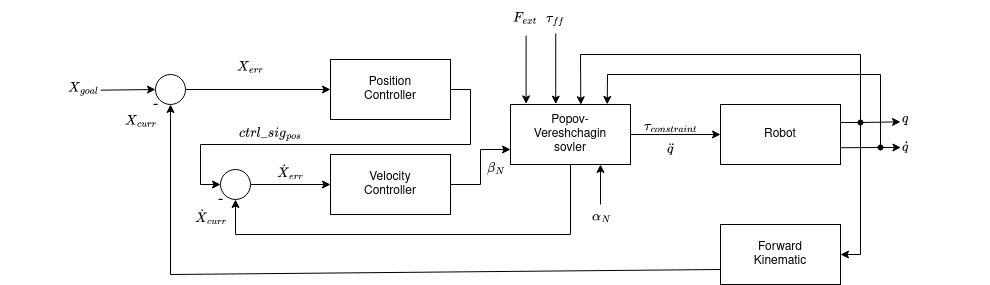
\includegraphics[width=1\linewidth]{images/systemdia.png}
        \caption{A generic control diagram illustrate the interactions of end-effector (task)
        pos and cascaded controllers with the constrained dynamics
        algorithm. It shows the connection between controller, solver and robot.}
        \label{fig:sys}
    \end{figure}
    \section{Extension of Robif2b}
\end{document}
